\RequirePackage[l2tabu, orthodox]{nag}
\documentclass[12pt]{article}

\usepackage[margin=1.9cm, letterpaper]{geometry}
\usepackage[utf8]{inputenc}
\usepackage{siunitx}
\usepackage{multicol}
\usepackage{mathtools}
\usepackage{amssymb}
\usepackage{mathrsfs}
\usepackage{graphicx}
\usepackage[outputdir=obj]{minted}
\usepackage{pdflscape}
\usepackage{caption}
\usepackage{subcaption}
\usepackage{epstopdf}
\usepackage{pgfplots}
\usepackage{pgfplotstable}
\usepackage{pdfpages}
\usepackage{indentfirst}
\usepackage{parskip}
\usepackage{booktabs}
\usepackage{float}
\usepackage{microtype}

\epstopdfsetup{outdir=./obj/}
\usemintedstyle{emacs}
\setminted{linenos,breaklines}

\setlength{\parskip}{1em}
\setlength{\parindent}{2em}

\pgfplotsset{compat=1.17}

\title{Transistor Amplifier}
\author{Hans Jarales (1537516) Michael Kwok (1548454)}
\date{November 3, 2020}
\begin{document}
\begin{titlepage}
\maketitle
\section{Abstract}
This Transistor Audio Amplifier design is a Two-Stage BJT-based Audio Amplifier. The purpose of this part of the project was to learn the utilization of transistors to function under certain objectives -- in this case, an audio amplifier application.

Three different Bipolar Junction Transistor configurations were examined and compared to achieve desired results. The configurations were: Common-Base, Common-Collector, Common-Emitter. In the end, to meet the required parameters defined for us, the Common Emitter and Common Collector stages were chosen after careful consideration. 

While the CE amplifier provides a desirable voltage gain, the input impedance experienced by the stage is much smaller than the required $R_{in}$. Accordingly, the CC amplifier is used after the input to boost the input impedance, allowing the amplifier fit to fit the required $R_{in}$, producing almost unity gain, allowing us to stay close to the desired voltage gain with the CE stage.

Our signatures certify that we are submitting our own, original work only, and do so in accordance with the University Code of Student Behaviour and APEGA's Code of Ethics.


\includegraphics[width=0.2\linewidth]{Lab1/hanssignature.png}
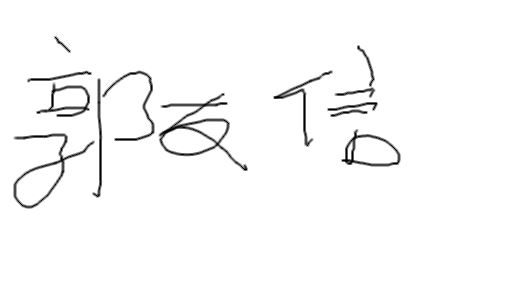
\includegraphics[width=0.2\linewidth]{Lab1/bepis.png}

\end{titlepage}
\newpage

\section{Objectives}
The Transistor Amplifier project aims to fulfill the following goals:
\begin{itemize}
    \item operation at 2kHz,
    \item produces a mid-band voltage gain of $12V/V \pm 5\%$,
    \item input impedance $R_{in} > 9k\Omega$,
    \item and a maximum output voltage swing of $9V_{pk-pk}$ without clipping.
\end{itemize}

\section{Design}
In order to meet the desired goals, a multi-stage amplifier was required, with \textit{maximum power transfer} in mind: one stage to address the low input impedance, and another stage to meet the desired voltage gain of $12V/V$.

The design approach begins from the output of the circuit to the input. Beginning with what is known, in this case, the load (a 1200:8$\Omega$ impedance transformer driving a 8$\Omega$ speaker), a BJT mode is chosen to accommodate the desired output voltage. Then, the next BJT stage is chosen to meet the input impedance requirement, accordingly.

Each stage is built and tested individually, making sure each respective stage meets desired operation. This modular design process streamlined troubleshooting -- allowing us to detect problems that occurred during testing real circuits against expected results via simulation, and theoretical values produced through calculation. Building and testing both stages together in unison would have increased the difficulty in troubleshooting in the event that undesired results present themselves. The ability to distinguish problems in the circuit becomes apparent when testing stages individually -- while testing the complete circuit removes this ability. Additionally, in this individual design process, several ideas and edits can be made and evaluated before joining the whole circuit.

The following three BJT amplification circuits were considered, along with their characteristics:


\begin{table}[htb]
    \caption{BJT Amplification Modes}
    \centering
    \begin{tabular}{c c c c}
        \toprule
                        & CE              & CC            & CB            \\
        \midrule
        Voltage Gain    &  \( > 10 V/V\)  & \( <1 V/V\)   & \( >20 V/V\)  \\
        Current Gain    & High \( \approx 10 \times\) & Very High     & Very Low  \\
        Input Impedance &  Medium         & High   & Very Low  \\
        Output Impedance    &  Medium  & Low-Medium   & Medium  \\
        \bottomrule
    \end{tabular}
    \label{tbl:1}
\end{table}


\subsection{Common Emitter Amplifier Stage}
For the desired mid-band voltage gain of $12V/V$, the Common Emitter (\textbf{CE}) Amplifier was chosen, with a desired voltage gain of $A_v \approx 13V/V$, slightly higher than required to address the voltage attenuation from the CC stage. The CE mode, produces a voltage gain that is relatively moderate compared to a Common Base amplifier, as shown in table \ref{tbl:1}, but was chosen as input impedance of this stage could be matched to the output impedance of the CC stage.

For \textit{maximum power transfer}, the load resistance $R_L$ must be equal to $R_C$. Since the $R_{out}$ of the CE stage is $1.2k\si{\ohm}$, $R_L = R_C = 1.2k\si{\ohm}$. For the CE stage, the voltage gain is found by:
$$A_v = \frac{R_C || R_L}{r_e + R_E} = 13V/V$$

Where $r_e = \frac{25mV}{i_E} = \frac{25mV}{i_C}$. Using KVL, we obtain $V_C = 9V - i_cR_c = 0$, and $i_C = \frac{9V}{1.2k\si{\ohm}} = 7.5mA$, and $r_e = \frac{25mV}{7.5mA} = 10/3\si{\ohm}$. Consequently, $R_E$ is found:
$$R_E = \frac{R_C||R_L}{A_v} - r_e = \frac{1.2k\si{\ohm} || 1.2k\si{\ohm}}{13} - 10/3\si{\ohm} = 42.8\si{\ohm}$$

Finding the DC voltage $V_E$: using KVL gives: $V_E = i_ER_E - 9V = 7.5mA \cdot 42.8\si{\ohm} - 9V = -8.68V$.

Using the relationship for BJT's in \textit{Forward Active Mode}, $V_{BE} = V_B - V_E = 0.7V$, consequently, $V_B = V_{BE} + V_E = 0.7V - 8.68V = -7.98V$.

Obtaining the bias current $i_{bias} = \frac{i_C}{10} = \frac{7.5mA}{10} = 750\mu A$

The bias resistors $R_{B1}$ and $R_{B2}$ can now be calculated.
Using KVL obtains: 

$V_{RB1} = 9 - V_B = 17.68V = i_{bias}\cdot R_{B1}$, and $R_{B1} =\frac{17.68V}{750\mu A } = 23.57k\Omega$.

$V_{RB2} = 9 + V_B = 1.02V = i_{bias}\cdot R_{B2}$ and $R_{B2} = \frac{1.02V}{750\mu A} = 1360\Omega$


\subsection{Common Collector Amplifier Stage}
For the high input impedance requirement, the Common Collector (\textbf{CC}) Amplifier is implemented as the first (input) stage. Important to recognize, however, is that the voltage gain of the CC amplifier is $A_v \approx 0.98$. In this case, there is no $R_C$, and hence for maximum voltage gain, $V_E$ is situated in between $\pm 9V$.

Given $i_{C-peak} = \frac{4.5V}{1.2k\Omega || 1.2k\Omega} = 7.5mA$.
$$i_{C-max, CE} = I_{C, DC} + i_{C-peak} = 2 \cdot 7.5mA = 15mA$$
$$i_{C-max, CC} = 25mA - i_{C-max, CE} = 10mA$$
$$I_{C-dc, CC} = \frac{i_{C-max, CC}}{2} - 1mA = 4mA$$
and $I_C = I_E$.
Therefore $R_E = \frac{9V}{I_E} = \frac{9V}{4mA} = 2250\Omega$
Obtaining the bias current; $$I_{bias} = \frac{I_C}{10} = 0.4mA$$
The bias resistors $R_{B1}$ and $R_{B2}$ can now be calculated.
Noting $V_E = 0$ Using KVL obtains:
$$V_{RB1} = 9V - V_{BE} = 9V - 0.7V = 8.3V$$
$$R_{B1} = \frac{V_{RB1}}{I_{bias}} = \frac{8.3V}{0.4mA} = 20.8k\Omega$$
$$V_{RB2} = 9V + 0.7V = 9.7V$$
$$R_{B2} = \frac{V_{RB2}}{I_{bias}} = \frac{9.7V}{0.4mA} = 24.3k\Omega$$

Since $R_L = R_{In, CE} = 1k\Omega$, and $r_e = \frac{25mV}{i_E} = \frac{25mV}{4mA} = 6.25\Omega$ solving for $A_v = \frac{R_E || R_L}{r_e + R_E||R_L}$
$$A_v = \frac{2250\Omega || 1000\Omega}{6.25\Omega(2250\Omega || 1000\Omega)} = 0.9991V/V$$

Solving for the input impedance using the calculated values and the formula
$$R_{in} = R_{B1} || R_{B2}||[(\beta+1)(r_e + R_E)]$$
$$R_{B1} || R_{B2} = 20.8k\Omega || 24.3k\Omega = 11207\Omega$$
$$r_e || R_E = 6.25\Omega || 2250\Omega = 692.31\Omega$$
$$R_{in} = (11207\Omega)\cdot[(100 + 1)\cdot(692.31)] = 9670.86\Omega$$

Indeed, the input impedance meets requirement: $R_{in} = 9670.86\si{\ohm} > 9k\si{\ohm}$.

\section{Simulation}

\subsection{Michael Kwok}

\begin{figure}[H]
    \centering
    \begin{subfigure}{0.45\textwidth}
        \centering
    \caption{CE stage DC Bias}
    \begin{tikzpicture}
        \begin{axis}[
            xlabel = Time (\si{\second}),
            ylabel = Voltage (\si{\volt}),
            xmajorgrids,
            ymajorgrids,
            yminorgrids,
            legend style = {at={(0.98, 0.7)},anchor=north east},
            xmin = 0,
            xmax = 0.0005,
            width = {0.9\linewidth}]
            \addplot table [x=time, y=V(n002), col sep=tab, mark=none] {CE.txt};
            \addlegendentry{$V_C$}
            \addplot table [x=time, y=V(n005), col sep=tab, mark=none] {CE.txt};
            \addlegendentry{$V_B$}
            \addplot table [x=time, y=V(n007), col sep=tab, mark=none] {CE.txt};
            \addlegendentry{$V_E$}
        \end{axis}
    \end{tikzpicture}
    \end{subfigure}
        \begin{subfigure}{0.45\textwidth}
            \centering
            \caption{CC stage DC Bias}
            \begin{tikzpicture}
                \begin{axis}[
                    xlabel = Time (\si{\second}),
                    ylabel = Voltage (\si{\volt}),
                    xmajorgrids,
                    ymajorgrids,
                    yminorgrids,
                    legend style = {at={(0.98, 0.7)},anchor=north east},
                    xmin = 0,
                    xmax = 0.0005,
                    width = {0.9\linewidth}]
                \addplot table [x=time, y=V(n001), col sep=tab, mark=none] {CC.txt};
                \addlegendentry{$V_C$}
                \addplot table [x=time, y=V(n003), col sep=tab, mark=none] {CC.txt};
                \addlegendentry{$V_B$}
                \addplot table [x=time, y=V(n005), col sep=tab, mark=none] {CC.txt};
                \addlegendentry{$V_E$}
                \end{axis}
            \end{tikzpicture}
    \end{subfigure}
    \caption{DC Biases}
    \label{grph:dcbias}
\end{figure}

As shown in Figure 1, the bias points are as the following:

\begin{table}[H]
    \centering
    \begin{tabular}{c c c}
    \toprule
           & CE                 & CC  \\
        \midrule
        \(V_C\) & \SI{0}{\volt}& \SI{9}{\volt}      \\
        \(V_B\) & \SI{-8.0}{\volt}& \SI{0.428}{\volt}   \\
        \(V_E\) & \SI{-8.64}{\volt}& \SI{-2.36}{\volt}  \\
    \bottomrule
    \end{tabular}
\end{table}

\begin{figure}[h]
    \centering
    \begin{subfigure}{0.45\textwidth}
    \caption{CE stage input and output}
    \begin{tikzpicture}
        \begin{axis}[
            xlabel = Time (\si{\second}),
            ylabel = Voltage (\si{\volt}),
            xmajorgrids,
            ymajorgrids,
            yminorgrids,
            legend pos = south east,
            xmin = 0,
            xmax = 0.0005,
            width = {0.9\linewidth}]
            \addplot table [x=time, y=V(n003), col sep=tab, mark=none] {CEGain.txt};
            \addlegendentry{\(V_{out}\)}
            \addplot table [x=time, y=V(n004), col sep=tab, mark=none] {CEGain.txt};
            \addlegendentry{\(V_{in}\)}
        \end{axis}
    \end{tikzpicture}
    \end{subfigure}
        \begin{subfigure}{0.45\textwidth}
        \caption{CE stage \(9\si{V}_{pp}\)}
    \begin{tikzpicture}
        \begin{axis}[
            xlabel = Time (\si{\second}),
            ylabel = Voltage (\si{\volt}),
            xmajorgrids,
            ymajorgrids,
            yminorgrids,
            xmin = 0,
            xmax = 0.0005,
            width = {0.9\linewidth}]
            \addplot table [x=time, y=V(n003), col sep=tab, mark=none] {CEClip.txt};
        \end{axis}
    \end{tikzpicture}
    \end{subfigure}
    \caption{CE Gain characteristics}
    \label{grph:cegain}
\end{figure}

In the figure on the left of Figure 2 the maximum input voltage recorded in the SPICE simulation was \SI{99.9}{\milli\volt}, and maximum output voltage was \SI{1.27}{\volt}. This means a gain of \SI[per-mode=symbol]{12.7}{\volt\per\volt} was observed, which is close to the target of \SI[per-mode=symbol]{13}{\volt\per\volt}

The other figure shows the output of the CE stage with a maximum voltage of \SI{4.29}{\volt} and a minimum voltage of \SI{-5.18}{\volt} which is \(9.78 \si{\volt}_{pp}\), and as show it does not clip.

    \begin{figure}[H]
    \centering
    \caption{\(\si{\volt}_x\) with \(R_{var} = 1150\si{\ohm}\)}
    \label{grph:ceimpede}
    \begin{tikzpicture}   
        \begin{axis}[
            xlabel = Time (\si{\second}),
            ylabel = Voltage (\si{\volt}),
            xmajorgrids,
            ymajorgrids,
            yminorgrids,
            xmin = 0,
            xmax = 0.0005,
            height = 7.5cm,
            width = {0.9\linewidth}]
            \addplot table [x=time, y=V(n004), col sep=tab, mark=none] {CERin.txt};
            \addlegendentry{\(V_in\)}
            \addplot table [x=time, y=V(n005), col sep=tab, mark=none] {CERin.txt};
            \addlegendentry{\(V_x\)}
        \end{axis}
    \end{tikzpicture}
    \end{figure}
    
To get the above graph, a \SI{1150}{\ohm} resistor was placed in series to the input voltage source which was set at \SI{100}{\milli\volt} and \SI{2}{\kilo\hertz}. As shown, \(V_x\) is half of \(V_{in}\), and so the input impedance is deduced to be \SI{1150}{\ohm}


\begin{figure}[H]
    \centering
    \begin{tikzpicture}
        \begin{axis}[
            title = {CC stage output and input},
            xlabel = Time (\si{\second}),
            ylabel = Voltage (\si{\volt}),
            xmajorgrids,
            ymajorgrids,
            yminorgrids,
            xmin = 0,
            xmax = 0.0005,
            height = 7.5cm,
            width = {0.9\linewidth}]
            \addplot table [x=time, y=V(n005), col sep=tab, mark=none] {CCGain.txt};
            \addlegendentry{\(V_{out}\)}
            \addplot table [x=time, y=V(n002), col sep=tab, mark=none] {CCGain.txt};
            \addlegendentry{\(V_{in}\)}
        \end{axis}
    \end{tikzpicture}
\end{figure}

As can be seen, the Gain/Attenuation in the CC stage is minimal and very close to unity. This is expected and intentional. Maximum input voltage recorded in the SPICE simulation was \SI{99.9}{\milli\volt}, and maximum output voltage was \SI{98.0}{\milli\volt}. This means a gain of \SI[per-mode=symbol]{0.98}{\volt\per\volt} was observed.

\begin{figure}[H]
    \centering
    \begin{tikzpicture}
        \begin{axis}[
            title = {\si{\volt} with \(R_{var} = 9670\si{\ohm}\)},
            xlabel = Time (\si{\second}),
            ylabel = Voltage (\si{\volt}),
            xmajorgrids,
            ymajorgrids,
            yminorgrids,
            xmin = 0,
            xmax = 0.0005,
            height = 7.5cm,
            width = {0.9\linewidth}]
            \addplot table [x=time, y=V(n003), col sep=tab, mark=none] {CCRin.txt};
            \addlegendentry{\(V_{x}\)}
            \addplot table [x=time, y=V(n002), col sep=tab, mark=none] {CCRin.txt};
            \addlegendentry{\(V_{in}\)}
        \end{axis}
    \end{tikzpicture}
\end{figure}

The required resistance to half the input voltage for the CC stage was \SI{9670}{\ohm}, which means that the input impedance is about \SI{9670}{\ohm}.

\begin{figure}[H]
    \centering
    \begin{subfigure}{0.45\textwidth}
    \caption{Combined input and output}
    \begin{tikzpicture}
        \begin{axis}[
            xlabel = Time (\si{\second}),
            ylabel = Voltage (\si{\volt}),
            xmajorgrids,
            ymajorgrids,
            yminorgrids,
            legend pos = south east,
            xmin = 0,
            xmax = 0.0005,
            width = {0.9\linewidth}]
            \addplot table [x=time, y=V(n002), col sep=tab, mark=none] {AllGain.tsv};
            \addlegendentry{\(V_{in}\)}
            \addplot table [x=time, y=V(n005), col sep=tab, mark=none] {AllGain.tsv};
            \addlegendentry{\(V_{out}\)}
        \end{axis}
    \end{tikzpicture}
    \end{subfigure}
        \begin{subfigure}{0.45\textwidth}
        \caption{Combined \(9\si{V}_{pp}\)}
    \begin{tikzpicture}
        \begin{axis}[
            xlabel = Time (\si{\second}),
            ylabel = Voltage (\si{\volt}),
            xmajorgrids,
            ymajorgrids,
            yminorgrids,
            legend pos = south east,
            xmin = 0,
            xmax = 0.0005,
            width = {0.9\linewidth}]
            \addplot table [x=time, y=V(n002), col sep=tab, mark=none] {Allclip.txt};
            \addlegendentry{\(V_{in}\)}
            \addplot table [x=time, y=V(n005), col sep=tab, mark=none] {Allclip.txt};
            \addlegendentry{\(V_{out}\)}
        \end{axis}
    \end{tikzpicture}
    \end{subfigure}
    \caption{Combined gain characteristics}
\end{figure}

The combined gain of both stages is calculated to be \SI[per-mode=symbol]{12.6}{\volt\per\volt}. This is within the requirements provided. Maximum input voltage recorded in the SPICE simulation was \SI{99.9}{\milli\volt}, and maximum output voltage was \SI{1.26}{\volt}.

\begin{figure}[H]
    \centering
    \begin{tikzpicture}
        \begin{axis}[
            title = {\si{\volt} with \(R_{var} = 9760\si{\ohm}\)},
            xlabel = Time (\si{\second}),
            ylabel = Voltage (\si{\volt}),
            xmajorgrids,
            ymajorgrids,
            yminorgrids,
            xmin = 0,
            xmax = 0.0005,
            height = 7.5cm,
            width = {0.9\linewidth}]
            \addplot table [x=time, y=V(n003), col sep=tab, mark=none] {AllRin.txt};
            \addlegendentry{\(V_{x}\)}
            \addplot table [x=time, y=V(n002), col sep=tab, mark=none] {AllRin.txt};
            \addlegendentry{\(V_{in}\)}
        \end{axis}
    \end{tikzpicture}
\end{figure}

\subsection{Hans Jarales}

\begin{figure}[H]
    \centering
    \begin{subfigure}{0.45\textwidth}
        \centering
    \caption{CE stage DC Bias}
    \begin{tikzpicture}
        \begin{axis}[
            xlabel = Time (\si{\second}),
            ylabel = Voltage (\si{\volt}),
            xmajorgrids,
            ymajorgrids,
            yminorgrids,
            legend style = {at={(0.98, 0.7)},anchor=north east},
            xmin = 0,
            xmax = 0.0005,
            width = {0.9\linewidth}]
            \addplot table [x=time, y=V(n002), col sep=tab, mark=none] {CE.txt};
            \addlegendentry{$V_C$}
            \addplot table [x=time, y=V(n005), col sep=tab, mark=none] {CE.txt};
            \addlegendentry{$V_B$}
            \addplot table [x=time, y=V(n007), col sep=tab, mark=none] {CE.txt};
            \addlegendentry{$V_E$}
        \end{axis}
    \end{tikzpicture}
    \end{subfigure}
        \begin{subfigure}{0.45\textwidth}
            \centering
            \caption{CC stage DC Bias}
            \begin{tikzpicture}
                \begin{axis}[
                    xlabel = Time (\si{\second}),
                    ylabel = Voltage (\si{\volt}),
                    xmajorgrids,
                    ymajorgrids,
                    yminorgrids,
                    legend style = {at={(0.98, 0.7)},anchor=north east},
                    xmin = 0,
                    xmax = 0.0005,
                    width = {0.9\linewidth}]
                \addplot table [x=time, y=V(n001), col sep=tab, mark=none] {CC.txt};
                \addlegendentry{$V_C$}
                \addplot table [x=time, y=V(n003), col sep=tab, mark=none] {CC.txt};
                \addlegendentry{$V_B$}
                \addplot table [x=time, y=V(n005), col sep=tab, mark=none] {CC.txt};
                \addlegendentry{$V_E$}
                \end{axis}
            \end{tikzpicture}
    \end{subfigure}
    \caption{DC Biases}
    \label{grph:dcbias}
\end{figure}

As shown in Figure \ref{grph:dcbias}, the bias points are as the following:

\begin{table}[H]
    \centering
    \begin{tabular}{c c c}
    \toprule
           & CE                 & CC  \\
        \midrule
        \(V_C\) & \SI{0}{\volt}& \SI{9}{\volt}      \\
        \(V_B\) & \SI{-8.0}{\volt}& \SI{0.428}{\volt}   \\
        \(V_E\) & \SI{-8.64}{\volt}& \SI{-2.36}{\volt}  \\
    \bottomrule
    \end{tabular}
\end{table}

\begin{figure}[h]
    \centering
    \begin{subfigure}{0.45\textwidth}
    \caption{CE stage input and output}
    \begin{tikzpicture}
        \begin{axis}[
            xlabel = Time (\si{\second}),
            ylabel = Voltage (\si{\volt}),
            xmajorgrids,
            ymajorgrids,
            yminorgrids,
            legend pos = south east,
            xmin = 0,
            xmax = 0.0005,
            width = {0.9\linewidth}]
            \addplot table [x=time, y=V(n003), col sep=tab, mark=none] {CEGain.txt};
            \addlegendentry{\(V_{out}\)}
            \addplot table [x=time, y=V(n004), col sep=tab, mark=none] {CEGain.txt};
            \addlegendentry{\(V_{in}\)}
        \end{axis}
    \end{tikzpicture}
    \end{subfigure}
        \begin{subfigure}{0.45\textwidth}
        \caption{CE stage \(9\si{V}_{pp}\)}
    \begin{tikzpicture}
        \begin{axis}[
            xlabel = Time (\si{\second}),
            ylabel = Voltage (\si{\volt}),
            xmajorgrids,
            ymajorgrids,
            yminorgrids,
            xmin = 0,
            xmax = 0.0005,
            width = {0.9\linewidth}]
            \addplot table [x=time, y=V(n003), col sep=tab, mark=none] {CEClip.txt};
        \end{axis}
    \end{tikzpicture}
    \end{subfigure}
    \caption{CE Gain characteristics}
    \label{grph:cegain}
\end{figure}

In the figure on the left of Figure \ref{grph:cegain} the maximum input voltage recorded in the SPICE simulation was \SI{99.9}{\milli\volt}, and maximum output voltage was \SI{1.27}{\volt}. This means a gain of \SI[per-mode=symbol]{12.7}{\volt\per\volt} was observed, which is close to the target of \SI[per-mode=symbol]{13}{\volt\per\volt}

The other figure shows the output of the CE stage with a maximum voltage of \SI{4.29}{\volt} and a minimum voltage of \SI{-5.18}{\volt} which is \(9.78 \si{\volt}_{pp}\), and as show it does not clip.
    \begin{figure}[H]
    \centering
    \caption{\(\si{\volt}_x\) with \(R_{var} = 1150\si{\ohm}\)}
    \label{grph:ceimpede}
    \begin{tikzpicture}   
        \begin{axis}[
            xlabel = Time (\si{\second}),
            ylabel = Voltage (\si{\volt}),
            xmajorgrids,
            ymajorgrids,
            yminorgrids,
            xmin = 0,
            xmax = 0.0005,
            height = 7.5cm,
            width = {0.9\linewidth}]
            \addplot table [x=time, y=V(n004), col sep=tab, mark=none] {CERin.txt};
            \addlegendentry{\(V_in\)}
            \addplot table [x=time, y=V(n005), col sep=tab, mark=none] {CERin.txt};
            \addlegendentry{\(V_x\)}
        \end{axis}
    \end{tikzpicture}
    \end{figure}
    
To get the above graph, a \SI{1150}{\ohm} resistor was placed in series to the input voltage source which was set at \SI{100}{\milli\volt} and \SI{2}{\kilo\hertz}. As shown, \(V_x\) is half of \(V_{in}\), and so the input impedance is deduced to be \SI{1150}{\ohm}

\begin{figure}[H]
    \centering
    \begin{tikzpicture}
        \begin{axis}[
            title = {CC stage output and input},
            xlabel = Time (\si{\second}),
            ylabel = Voltage (\si{\volt}),
            xmajorgrids,
            ymajorgrids,
            yminorgrids,
            xmin = 0,
            xmax = 0.0005,
            height = 7.5cm,
            width = {0.9\linewidth}]
            \addplot table [x=time, y=V(n005), col sep=tab, mark=none] {CCGain.txt};
            \addlegendentry{\(V_{out}\)}
            \addplot table [x=time, y=V(n002), col sep=tab, mark=none] {CCGain.txt};
            \addlegendentry{\(V_{in}\)}
        \end{axis}
    \end{tikzpicture}
\end{figure}

As can be seen, the Gain/Attenuation in the CC stage is minimal and very close to unity. This is expected and intentional. Maximum input voltage recorded in the SPICE simulation was \SI{99.9}{\milli\volt}, and maximum output voltage was \SI{98.0}{\milli\volt}. This means a gain of \SI[per-mode=symbol]{0.98}{\volt\per\volt} was observed.

\begin{figure}[H]
    \centering
    \begin{tikzpicture}
        \begin{axis}[
            title = {\si{\volt} with \(R_{var} = 9670\si{\ohm}\)},
            xlabel = Time (\si{\second}),
            ylabel = Voltage (\si{\volt}),
            xmajorgrids,
            ymajorgrids,
            yminorgrids,
            xmin = 0,
            xmax = 0.0005,
            height = 7.5cm,
            width = {0.9\linewidth}]
            \addplot table [x=time, y=V(n003), col sep=tab, mark=none] {CCRin.txt};
            \addlegendentry{\(V_{x}\)}
            \addplot table [x=time, y=V(n002), col sep=tab, mark=none] {CCRin.txt};
            \addlegendentry{\(V_{in}\)}
        \end{axis}
    \end{tikzpicture}
\end{figure}

The required resistance to half the input voltage for the CC stage was \SI{9670}{\ohm}, which means that the input impedance is about \SI{9670}{\ohm}.

\begin{figure}[H]
    \centering
    \begin{subfigure}{0.45\textwidth}
    \caption{Combined input and output}
    \begin{tikzpicture}
        \begin{axis}[
            xlabel = Time (\si{\second}),
            ylabel = Voltage (\si{\volt}),
            xmajorgrids,
            ymajorgrids,
            yminorgrids,
            legend pos = south east,
            xmin = 0,
            xmax = 0.0005,
            width = {0.9\linewidth}]
            \addplot table [x=time, y=V(n002), col sep=tab, mark=none] {AllGain.tsv};
            \addlegendentry{\(V_{in}\)}
            \addplot table [x=time, y=V(n005), col sep=tab, mark=none] {AllGain.tsv};
            \addlegendentry{\(V_{out}\)}
        \end{axis}
    \end{tikzpicture}
    \end{subfigure}
        \begin{subfigure}{0.45\textwidth}
        \caption{Combined \(9\si{V}_{pp}\)}
    \begin{tikzpicture}
        \begin{axis}[
            xlabel = Time (\si{\second}),
            ylabel = Voltage (\si{\volt}),
            xmajorgrids,
            ymajorgrids,
            yminorgrids,
            legend pos = south east,
            xmin = 0,
            xmax = 0.0005,
            width = {0.9\linewidth}]
            \addplot table [x=time, y=V(n002), col sep=tab, mark=none] {Allclip.txt};
            \addlegendentry{\(V_{in}\)}
            \addplot table [x=time, y=V(n005), col sep=tab, mark=none] {Allclip.txt};
            \addlegendentry{\(V_{out}\)}
        \end{axis}
    \end{tikzpicture}
    \end{subfigure}
    \caption{Combined gain characteristics}
\end{figure}

The combined gain of both stages is calculated to be \SI[per-mode=symbol]{12.6}{\volt\per\volt}. This is within the requirements provided. Maximum input voltage recorded in the SPICE simulation was \SI{99.9}{\milli\volt}, and maximum output voltage was \SI{1.26}{\volt}.

\begin{figure}[H]
    \centering
    \begin{tikzpicture}
        \begin{axis}[
            title = {\si{\volt} with \(R_{var} = 9760\si{\ohm}\)},
            xlabel = Time (\si{\second}),
            ylabel = Voltage (\si{\volt}),
            xmajorgrids,
            ymajorgrids,
            yminorgrids,
            xmin = 0,
            xmax = 0.0005,
            height = 7.5cm,
            width = {0.9\linewidth}]
            \addplot table [x=time, y=V(n003), col sep=tab, mark=none] {AllRin.txt};
            \addlegendentry{\(V_{x}\)}
            \addplot table [x=time, y=V(n002), col sep=tab, mark=none] {AllRin.txt};
            \addlegendentry{\(V_{in}\)}
        \end{axis}
    \end{tikzpicture}
\end{figure}

\section{Experiment}
Standard resistor values were used to achieve closest to calculated values obtained in the \textbf{Design} section. Additionally, resistor values may have been manipulated to obtain desired results.

\subsection{Common Emitter Stage Results}
The DC bias voltages for the Common Emitter stage were obtained:
\begin{itemize}
    \item $V_E$ = -8.5V
    \item $V_B$ = -7.9V
    \item $V_C$ = -1.7V
\end{itemize}

\begin{figure}[H]
\centering
    \begin{subfigure}{.45\textwidth}
      \centering
      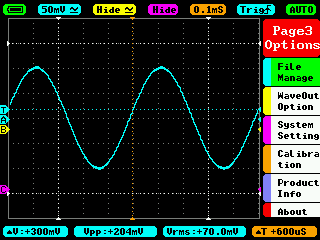
\includegraphics[width=\linewidth]{Lab2/CE_Vin.png}  
      \caption{$V_{in}$ of CE Stage using a $12k\Omega$ series resistance}
    \end{subfigure}
    \begin{subfigure}{.45\textwidth}
      \centering
      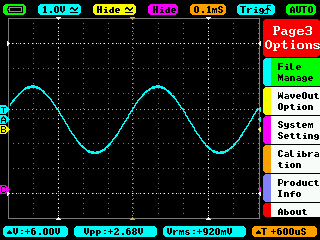
\includegraphics[width=\linewidth]{Lab2/CE_Vout.png}  
      \caption{$V_{out}$ of CE Stage}
    \end{subfigure}
    \caption{}
\end{figure}

Calculating for the actual voltage gain $A_v$,
$$A_v = \frac{V_{out}}{V_{in}} = \frac{2.68V_{pp}}{204mV_{pp}} = 13.039V/V$$
Using the calculated $R_E$ of around \SI{47}{\ohm} resulted in a gain that was much less than desired. Thus, $R_E$ was decreased to a resistor valued at around \SI{33}{\ohm}, increasing the gain $A_v$.

\subsection{Common Collector Stage Results}
The DC bias voltages for the Common Collector stage were obtained:
\begin{itemize}
    \item $V_E$ = -0.01V
    \item $V_B$ = 0.6V
    \item $V_C$ = 8.86V
\end{itemize}

\begin{figure}[H]
\centering
    \begin{subfigure}{.45\textwidth}
      \centering
      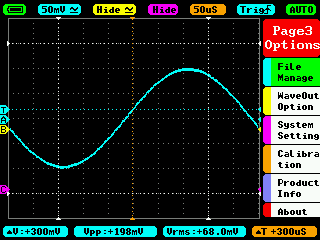
\includegraphics[width=\linewidth]{Lab2/CC_Vin.png}  
      \caption{$V_{in}$ of CC Stage}
    \end{subfigure}
    \begin{subfigure}{.45\textwidth}
      \centering
      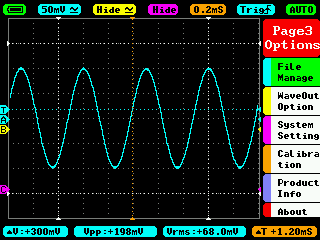
\includegraphics[width=\linewidth]{Lab2/CC_Vout.png}  
      \caption{$V_{out}$ of CC Stage}
    \end{subfigure}
\end{figure}

Note that the trigger (time scaling) were on different settings between the $V_{in}$ and $V_{out}$ wave forms. Indeed, the voltage gain of the CC stage is $A_v = = \frac{V_{out}}{V_{in}} =\approx 0.95V/V$.


A series resistance was used following the signal generator such that when the voltage $V_X$ became directly half of $V_{in} = 200mV$. This series resistance $R_{var}$ indicates then the input impedance $R_{in}$ of the CC Stage such that $R_{var} = R_{in}$.
\begin{figure}[H]
\centering
    \begin{subfigure}{.45\textwidth}
      \centering
      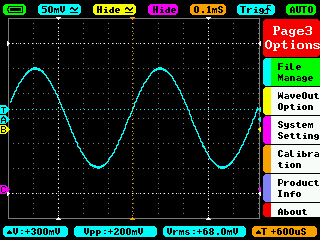
\includegraphics[width=\linewidth]{Lab2/SignalGenerator_Vin.png}  
      \caption{Signal Generation Waveform ($V_{in}$)}
    \end{subfigure}
    \begin{subfigure}{.45\textwidth}
      \centering
      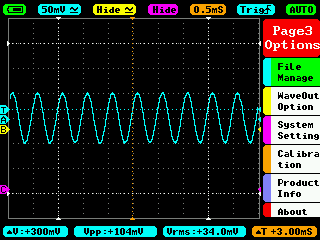
\includegraphics[width=\linewidth]{Lab2/V_X.png}  
      \caption{$V_X$ waveform}
    \end{subfigure}
    \caption{}
\end{figure}

The voltage waveform $V_X = \frac{1}{2}V_{in}$ was obtained using a $21.72k\Omega$ series resistance ($21k\Omega + 720\Omega$ connected in series). Thus, the actual input impedance is $R_{var} = R_{in} = 21.72k\Omega$ which indeed meets the objective $R_{in} > 9k\Omega$. Noted, however, is the great discrepancy between the calculated/theoretical input impedance of $R_{in} = 9760\Omega$ shown in the Design section. The overall circuit (both stages, coupled) achieved roughly the same waveform $V_X$, and therefore the $R_{in}$ was the same.

\begin{figure}[H]
    \centering
    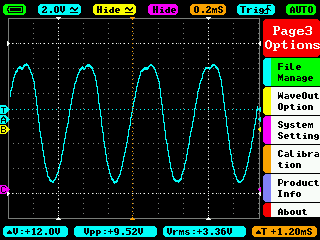
\includegraphics{Lab2/9VPP.png}
    \caption{Voltage waveform of overall circuit output voltage}
\end{figure}

The resulting $V_{out}$ above represents a 9.52$V_{pk-pk}$. Indeed, this meets the objective of having a $V_{out} \approx 9 V_{pk-pk}$.

\section{Discussion}
\begin{itemize}
    \item Does the order of the amplifier matter? Why?
    \begin{itemize}
        \item Yes the order does matter. If we exchanged the order for our amplifier as an example, the input impedance would not have been as high as required, and power transfer between stages would not have been optimal due to impedance mismatch.
    \end{itemize}
    \item Comment on the stability of your amplifier. Did you face instability problems? What modifications, if any, were needed to the design and/or the circuit?
    \begin{itemize}
        \item We did not seem to come across any instability issues with our amplification circuit.
    \end{itemize}
    \item What is the intent of the impedance transformer? Why is it necessary?
    \begin{itemize}
        \item The impedance transformer was necessary as the speaker we had was small, and likely had low impedance. For maximum power transfer, and thus audio volume, a reduction in impedance was needed.
    \end{itemize}
    \item Why is the high input impedance amplifier necessary?
    \begin{itemize}
        \item We require a high input impedance to reduce voltage drop due to the voltage divider effect. As shown in table \ref{tbl:1}, the CC stage is most suitable for this as it has inherently high input impedance due to the design of the amplifier.
    \end{itemize}
    \item In this lab we assumed that the input and output impedance is purely resistive. Is this a fair assumption? What are the issues with this assumption?
    \begin{itemize}
        \item While not perfect, it's a fair assumption as most of our components had resistive impedance, and capacitors were used to couple between stages instead of as impedance sources. Accounting for parasitic inductive and capacitive impedances would have made calculation harder and might not have made the results more accurate by much.
    \end{itemize}
    \item Were there any other difficulties you faced? What steps could you do to address these issues (even if you did not actually do them or could not do them)?
    \begin{itemize}
        \item Added resistance and capacitance from using a breadboard required us to use different resistor values from our simulations to arrive to similar results.
        \item Resistor values are not exactly the same as those we used in our simulations as in the real world, there are a set of existing resistor values, and it would not be realistic to make a \SI{5456}{\ohm} resistor for example. We had to combine multiple resistors in series to get close to our required values, but very few matched our simulation schematic directly.
    \end{itemize}
\end{itemize}
\section{Conclusion}
The design of a Transistor Amplifier requires the extensive knowledge and background behind the operation of Bipolar Junction Transistors, their different amplification modes, and their respective operating conditions.

As seen in this project, combining multiple stages of different BJT amplifier configurations might be required to fulfill the specified characteristics of a project. In this case, two different BJT amplifier stages were used (Common Collector, and Common Emitter) to address the different objectives of this project.

The most efficient, and effective design process is one that involves simulating, testing, and implementing each individual stage before their combination. This allows problems to be distinguished more easily and earlier on in the design, as opposed to a potential cascade of problems revealing themselves when constructing the total circuit. 

\newpage
\appendix

\section{Schematics}

\begin{figure}[H]
    \centering
    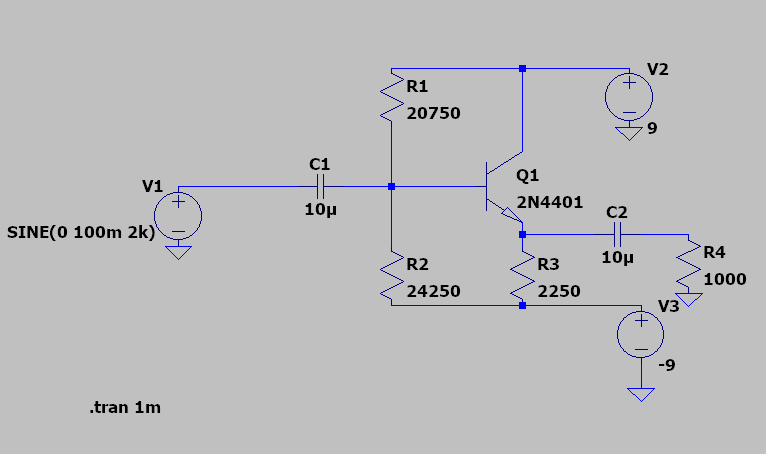
\includegraphics[width=\linewidth]{Lab2/CC.png}
    \caption{Common Collector Stage}
\end{figure}

\begin{figure}[H]
    \centering
    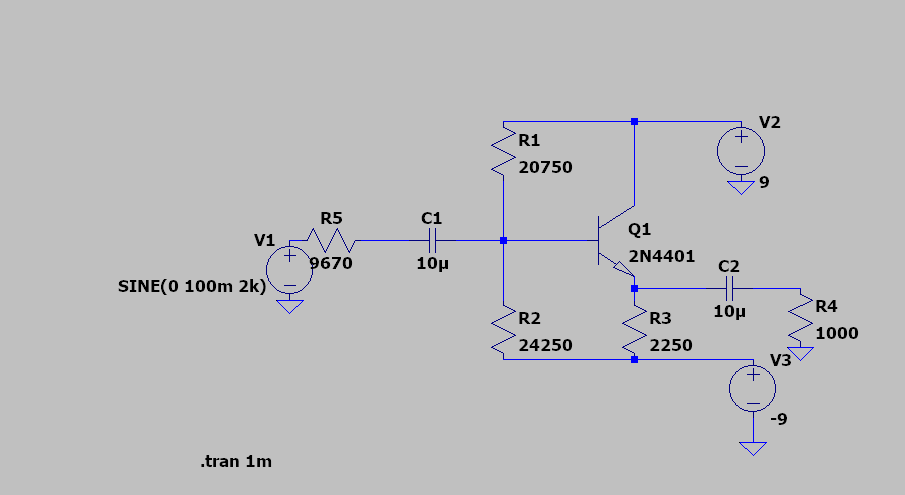
\includegraphics[width=\linewidth]{Lab2/CC_Rin.png}
    \caption{Common Collector Stage with \(R_{var}\)}
\end{figure}

\begin{figure}[H]
    \centering
    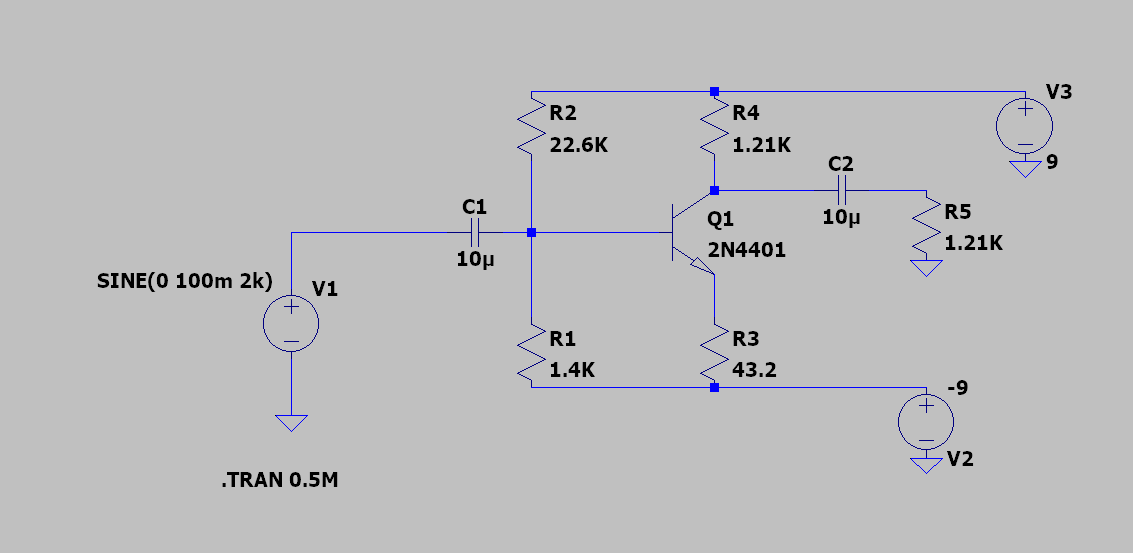
\includegraphics[width=\linewidth]{Lab2/CE.png}
    \caption{Common Emitter Stage}
\end{figure}

\begin{figure}[H]
    \centering
    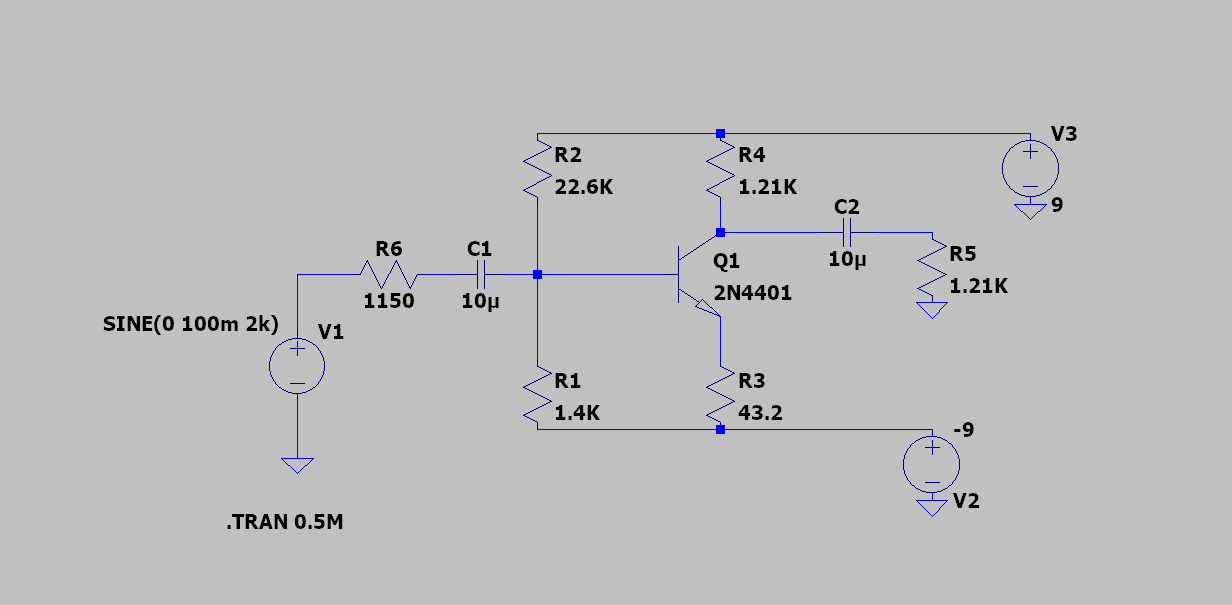
\includegraphics[width=\linewidth]{Lab2/CE_Rin.png}
    \caption{Common Emitter Stage with \(R_{var}\)}
\end{figure}

\begin{figure}[H]
    \centering
    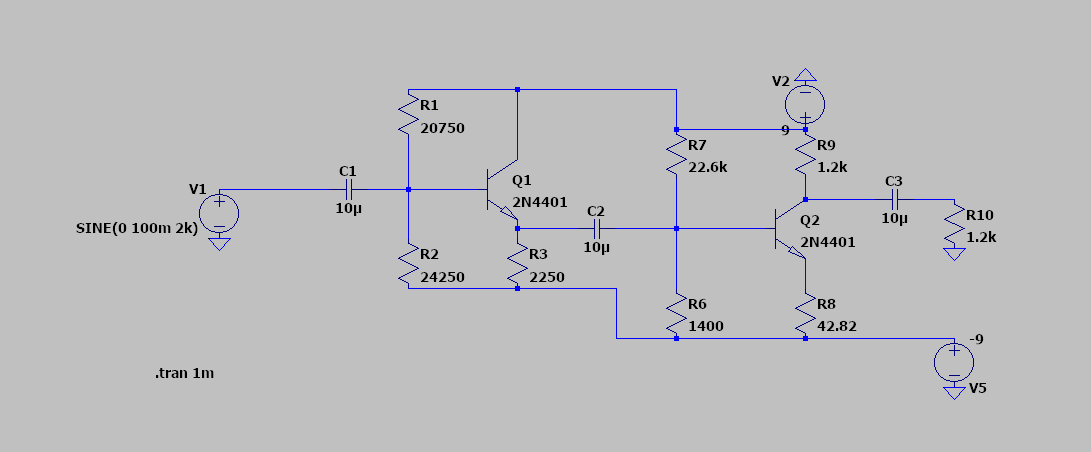
\includegraphics[width=\linewidth]{Lab2/All.png}
    \caption{Combined Amplifiers}
\end{figure}

\begin{figure}[H]
    \centering
    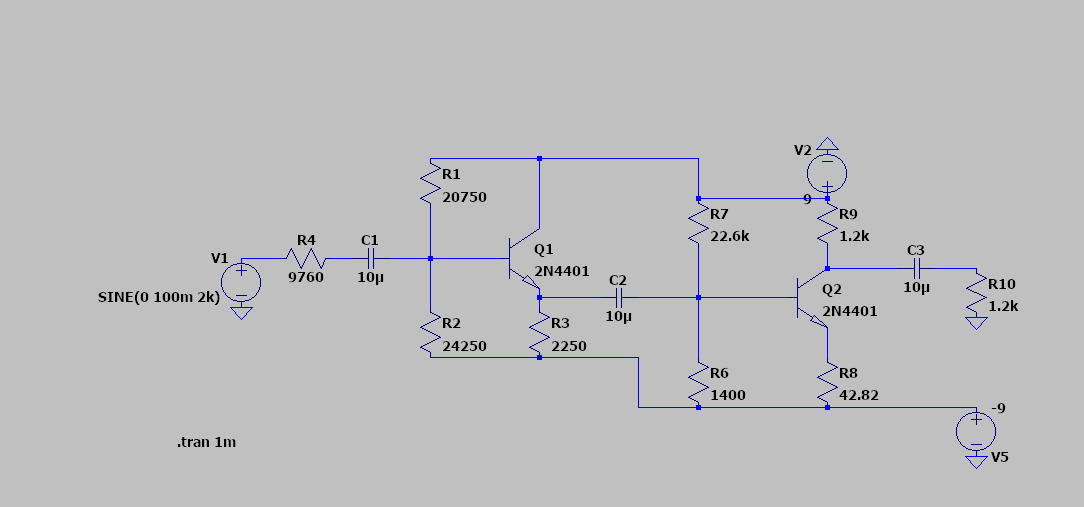
\includegraphics[width=\linewidth]{Lab2/All_Rin.png}
    \caption{Combined Amplifiers with \(R_{var}\)}
\end{figure}

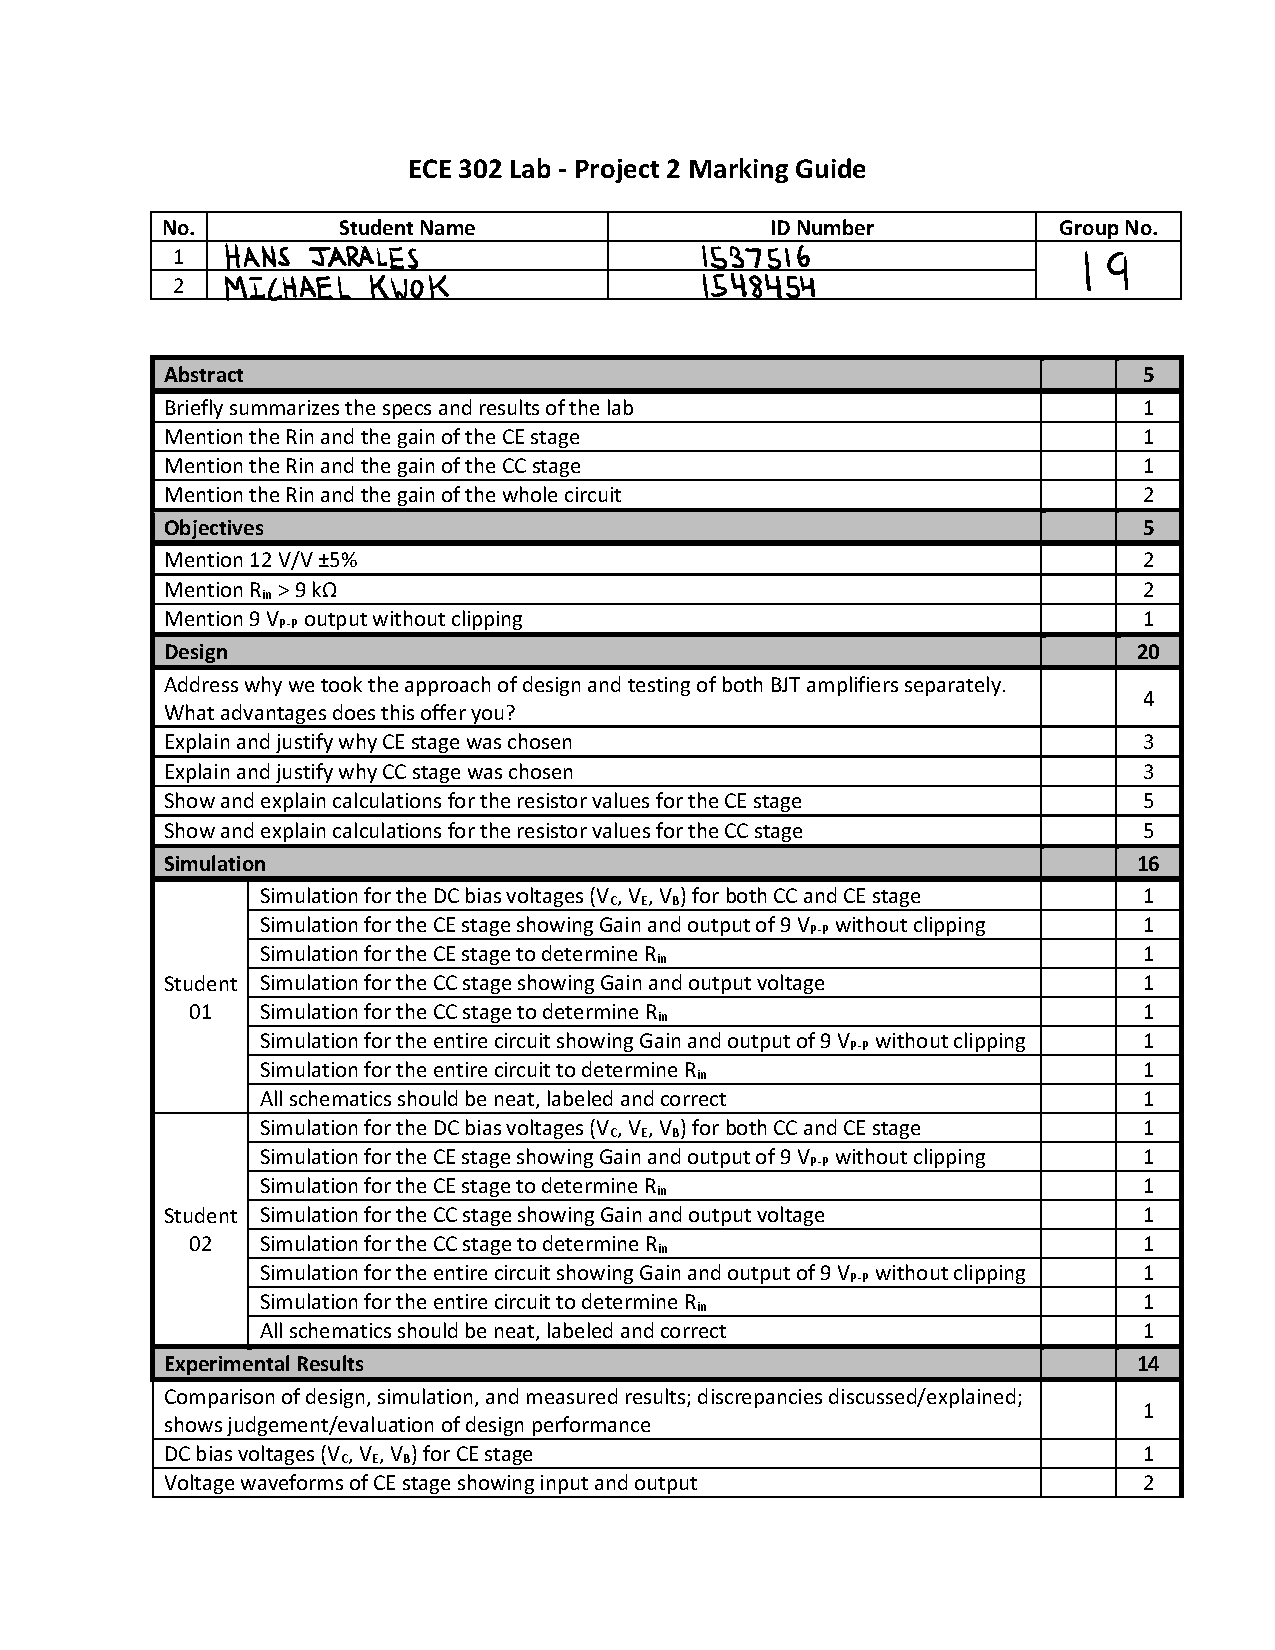
\includepdf[pages=-]{Lab2MarkingSheet.pdf}
\end{document}

